\chapter[Sistemas de recomendação]{Sistemas de recomendação}

Sistemas de recomendação são ferramentas computacionais e técnicas usadas para
produzir recomendação de itens úteis a um usuário \cite{mahmood2009improving}.
Sendo assim, um sistema de recomendação pode ser usado em diversos contextos,
desde melhorar a experiência de usuário a até mesmo melhorar a taxa de vendas
em uma aplicação comercial. Além disso, um sistema de recomendação também pode
ser usado para recomendar uma grande gama de itens, como filmes e livros
\cite{ricci2011introduction}. Para realizar a tarefa de recomendação, duas abordagens distintas podem ser usadas:
recomendação não-personalizadas e personalizadas.

Recomendações não-personalizadas são aquelas que não usam nenhuma informação do
usuário para realizar a recomendação. Exemplo de estratégias assim podem ser
visto em sites de música que apresentam a lista das 10 músicas mais
ouvidas. Já recomendações personalizadas, são aquelas que usam as avaliações já
realizadas por um usuário sobre um item para criar uma função preditiva que irá avaliar itens que ainda não foram
avaliados pelo usuário. Então, o sistema recomenda aqueles que possuem maior valor
apresentado pela função preditiva. A Figura \ref{fig:modelo_recomendacao} mostra
o processo para realizar uma recomendação personalizada \cite{picault2011get}.

\begin{figure}[h]
  \centering
  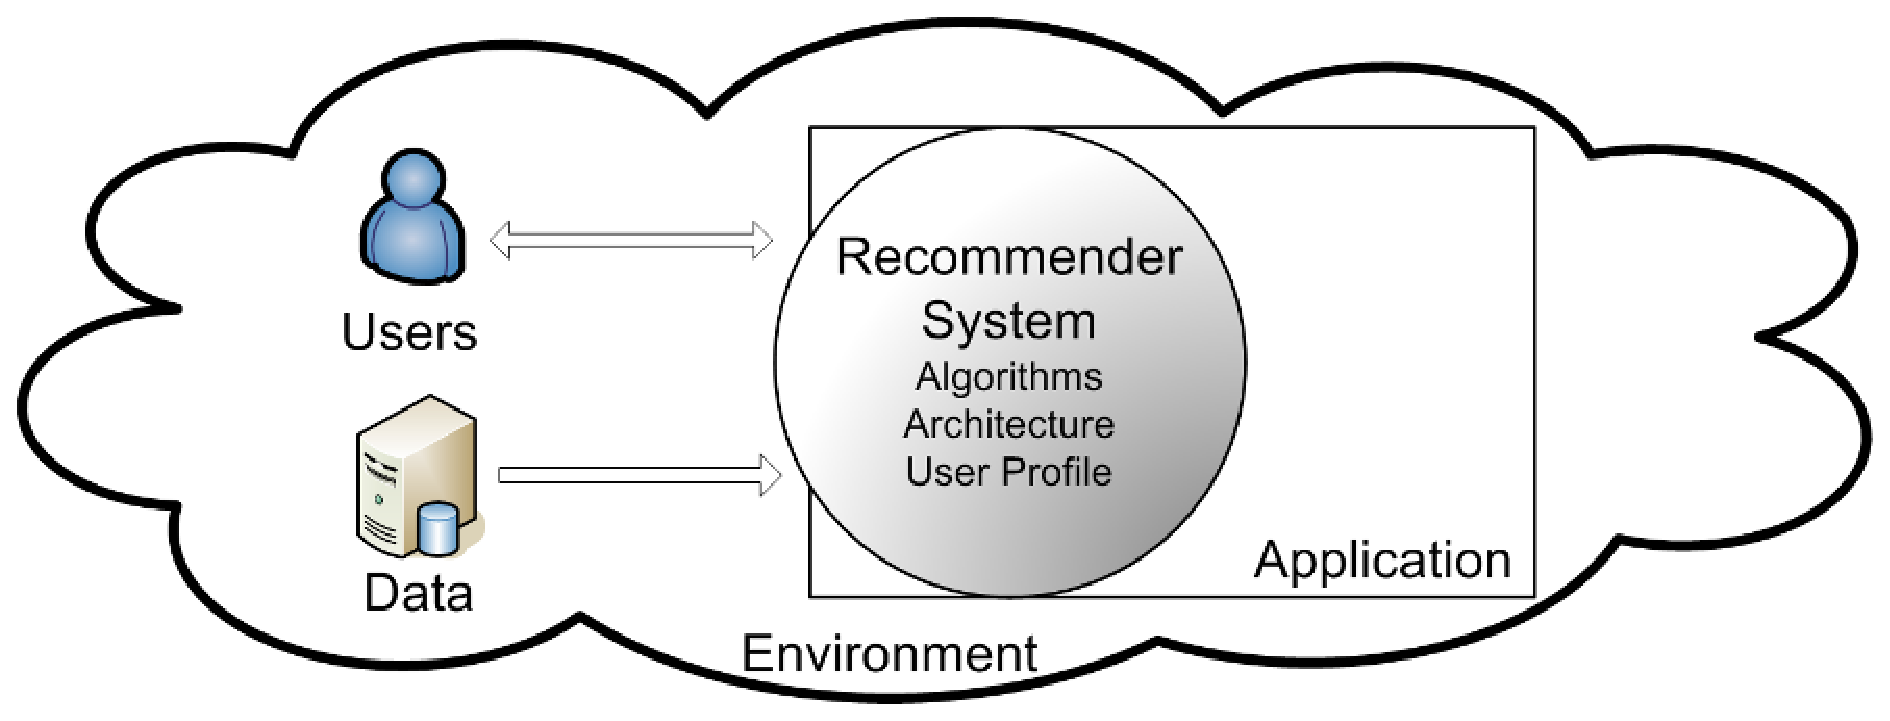
\includegraphics[width=0.9\textwidth]{figuras/recommender_model.eps}
  \caption{Modelo para criação de um sistema de recomendação personalizado}
  \label{fig:modelo_recomendacao}
\end{figure}

Pode-se ver na Figura \ref{fig:modelo_recomendacao} que as principais entradas
para um sistema de recomendação são os usuários do mesmo e os dados relacionados
a este mesmo usuário. No que tange o sistema de recomendação em si, pode-se
observar fatores importantes no design do mesmo, como o perfil do usuário, o
algoritmo de recomendação ou estratégia a ser usada e a infra-estrura a ser
usada. Além disso, nenhum sistema de recomendação está imune ao contexto no qual
o mesmo será usado.

Vale considerar que o perfil do usuário e a estratégia de recomendação usadas
são bastante dependentes um do outro. O perfil do usuário é a forma como o
usuário será representado no sistema, podendo ser gerado de inúmeras maneiras,
como uma lista de itens avaliados por exemplo. Sendo assim, características dos itens,
números de itens avaliados e a forma como o perfil do usuário é modelado são aspectos
fundamentais para a seleção de uma estratégia de recomendação, pois dependendo
da configuração desses atributos, algumas estratégias
de recomendação devem ser descartadas \cite{picault2011get}.

\section{Estratégias de recomendação} \label{sec:estrategias_recomendacao}

Com o conjunto de dados definidos, pode-se então escolher uma estratégia de
recomendação adequada. Para agrupar tais estratégias, considerou-se taxinomia de
alguns autores, como por exemplo \cite{burke2007hybrid}. As recomendações
descritas a seguir foram as que se mostraram mais presentes nas taxinomias
estudadas.

\begin{itemize}
    \item \textbf{Estratégias baseadas em conteúdo: } São aquelas que buscam
        recomendar itens similares ao que usuário já avaliou. A similiraridade
        dos itens é estimada pelos atributos que compõem um dado item no
        sistema. O fluxo de uma estratégia baseada em conteúdo pode ser vista na
        Figura \ref{fig:recomendacao_conteudo} \cite{lops2011content}.

        \begin{figure}[h]
            \centering
            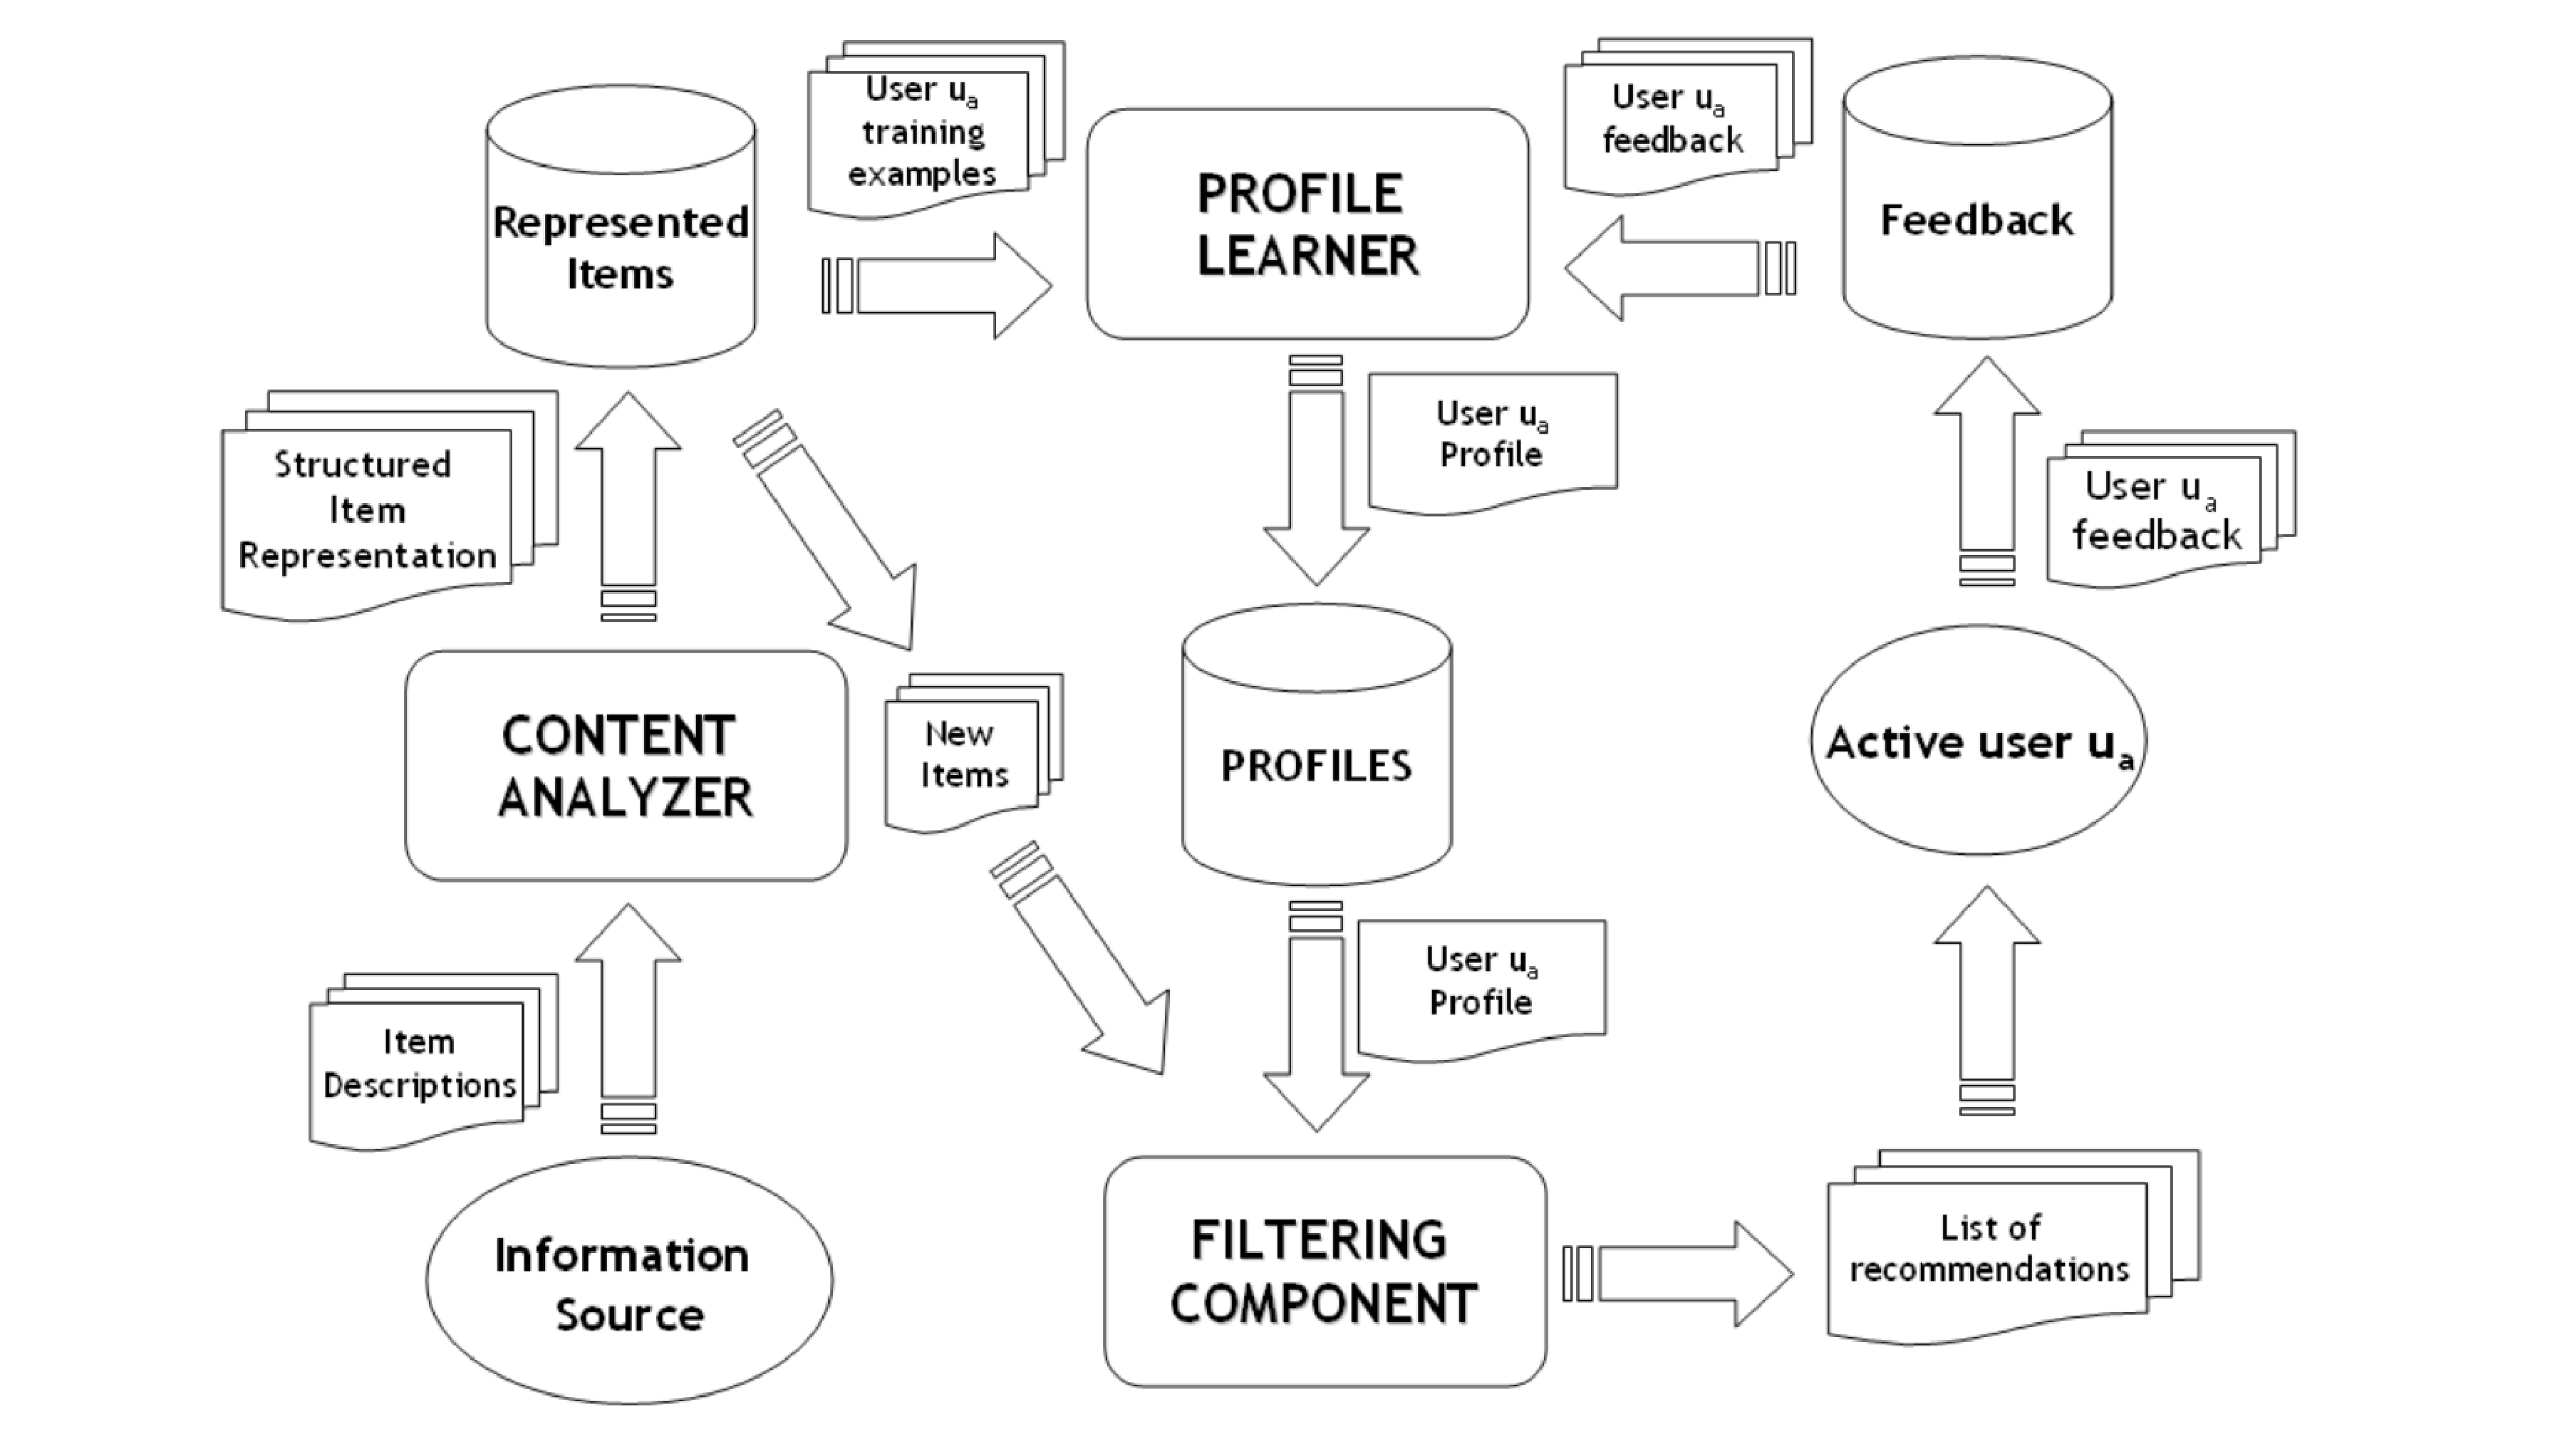
\includegraphics[width=0.9\textwidth]{figuras/recomendacao_conteudo}
            \caption{Fluxo para construção de um sistema de recomendação por
            conteúdo}
            \label{fig:recomendacao_conteudo}
        \end{figure}

        Pode-se ver pela Figura \ref{fig:recomendacao_conteudo} que uma recomendação
        por conteúdo se baseia fortemente em alguns itens chave. O
        \textit{Content Analyser} é a parte do sistema de recomendação que
        transforma os itens avaliados pelo usuário em entradas válidas para o
        algoritmo, ou seja, seleciona os atributos escolhidos do mesmo. O
        \textit{Profile Learner} é o responsável por criar o perfil do
        usuário, analisando os dados filtrados pelo \textit{Content Analyser} e
        criando um perfil de acordo com um modelo definido pelo sistema de
        recomendação. Uma técnica normalmente aplicada para essa tarefa é a
        \textit{Term Frequency-Inverse Term Frequency (TFIDF)} para selecionar
        os atributos de maior impacto nos itens avaliados pelo usuário, e então
        compor o perfil do usuário com tais termos \cite{lops2011content},
        essa técnica é explicada no Apêndice \ref{ape:tfidf}.  Por fim, o
        \textit{Filtering component} nada mais é do que uma ferramenta que recebe
        o perfil do usuário como entrada e usa o mesmo para filtrar os melhores
        itens que se aproximam desse perfil da base de dados possível. Sendo assim,
        a função preditiva desta estratégia de recomendação é uma combinação do
        perfil de usuário juntamente com uma forma de avaliar a similaridade entre
        dois itens.

        Dado essas características da recomendação baseada por conteúdo, pode-se
        perceber que a mesma pode sofrer o problema de superespecialização, já
        que podem haver dificuldades em classificar itens que nunca foram
        usados pelo usuário e também recomendar apenas itens próximos ao atual
        perfil do mesmo, dificultando assim a recomendação que podem vir a se
        tornar uma surpresa para o mesmo. \cite{lops2011content}.

    \item \textbf{Estratégias colaborativas:} Estratégias que recomendam itens
        de usuários com avaliações similares aos itens avaliados pelo usuário
        que está usando o sistema \cite{schafer2007collaborative}.
        Para determinar a similaridade de um usuário a outro, as avaliações de
        ambos são comparadas, visando assim encontrar usuários próximos um do
        outro. Uma vez definido a vizinhança do usuário, a recomendação de um
        item é normalmente feita por selecionar itens mais presentes no perfil
        dos vizinhos \cite{araujo2011apprecommender}. Vale ressaltar que este tipo de recomendação é uma das mais
        populares quando se trata de sistemas de recomendação
        \cite{ricci2011introduction}.

        Entretanto, vale ressaltar que esse tipo de estratégia necessita fortemente
        de uma ampla base de usuários para que a mesma possa ser aplicada. Isso
        se dá pela necessidade de criar uma vizinhança significativa de usuários
        com gostos similiares. Sendo assim, para aplicações que não possuem uma
        base de usuário relacionados ou até mesmo tratam do seu usuário de forma
        isolada, tal estratégia pode ter uma implementação bastante complicada.
        Além disso, outro problema é que essa estratégia tem um
        grande problema para recomendar itens que não possuem avaliações por
        nenhum usuário, o que dependendo da motivação usada para criar o sistema
        de recomendação, pode vir a se tornar um problema.
        \cite{ricci2011introduction}.


    \item \textbf{Estratégias híbridas: } Estratégias que combinam uma ou mais
        estratégias para gerarem uma recomendação. Normalmente tais estratégias
        são combinadas para que os pontos fracos de uma estratégia sejam
        suavizados pela outra. Por exemplo, combinar estratégias colaborativas com
        baseadas em conteúdo pode resolver problemas de superespecialização
        gerados por estratégias baseadas em conteúdo e também resolver problemas
        de recomendação de itens que ainda não foram avaliados, o que não
        acontece em recomendações baseadas em conteúdo.

\end{itemize}


\section{Contexto em sistemas de recomendação}

Apesar dos modelos apresentados na Seção \ref{sec:estrategias_recomendacao}
serem bastante distintos um do outro, cada um deles pode usar algumas
abordagens diferenciadas para tornar o perfil do usuário mais próximo à
realidade. Para isso, uma abordagem que pode ser usada é a de recomendação
baseada em contexto. Para esta recomendação, os itens avaliados pelo usuário são
combinados com informações de contexto do próprio usuário. Segundo \citeonline{berry1997data},
contexto pode ser definido como uma informação que caracteriza os estágios de
vida de um usuário e que pode determinar mudanças de preferências e status
do mesmo. Informações de contexto podem ser obtidas de forma implícita ou até
mesmo serem subentendidas pelo sistema, podendo assim gerar novos atributos
interessantes para o perfil do usuário. Um exemplo de informação contextual
seria o tempo no qual um usuário realizou a avaliação de um item. Um sistema de
recomendação pode usar essa informação para priorizar avaliações mais recentes
do que mais antigas, visando manter um perfil mais atualizado do usuário.

Sendo assim, para adicionar informação contextual em um sistema de recomendação
personalizado, três abordagens distintas são propostas por
\citeonline{adomavicius2011context}:

\begin{itemize}
    \item \textbf{Pré-filtragem: } As informações que serão usadas
        para realizar uma recomendação são pré-filtradas por informações de
        contexto antes de alimentarem o sistema de recomendação. Um exemplo
        dessa abordagem pode ser quando um sistema de recomendação só deseja
        receber as avaliações mais recentes do usuário, usando informação
        temporal de contexto para filtrar itens avaliados a muito tempo.
    \item \textbf{filtragem pós recomendação: } Após uma recomendação ter sido
        executada, os itens recomendados são filtrados por informações
        contextuais. Por exemplo, supondo que um usuário esteja procurando
        sugestões de restaurantes, o sistema pode fazer essa sugestão e usar a
        localização do usuário para retirar restaurantes muito longes da sua
        localização atual.
    \item \textbf{Modelagem contextual: } As informações contextuais são usadas
        para modelar o perfil do usuário ou até mesmo afetar como o perfil do
        usuário será criado.
\end{itemize}

\section{Avaliação de recomendadores}

Sistemas de recomendação podem ser avaliados de duas maneiras, que vão desde
experimentos de comparação offline, que usam uma base de dados previamente
coletada para serem executados, a até mesmo experimentos com usuários, que visam
averiguar questões mais subjetivas do recomendador.

Visto a subjetividade intrínseca de um sistema de recomendação, pode-se entender
que experimentos de usuários podem prover respostas bastante significativas para
algumas questões, entretanto a sua preparação e execução deve ser analisada mais
profundamente.

\subsection{Experimentos com usuário}

Para experimentos com usuários, um conjunto de usuários é selecionado, visando
a interação dos mesmos com o sistema, de forma que eles sejam capazes de responder algumas
questões objetivas e até mesmo subjetivas quanto ao processo de recomendação e
os próprios itens sendo recomendados.

Entretanto, vale ressaltar que este tipo de experimento apresenta algumas
dificuldades. A primeira delas está no custo de se fazer um experimento dessa
forma, pois além de fatores como seleção de usuário e isolar um ambiente de
teste, tornar tais experimentos repetíveis pode-se tornar bastante complexo
\cite{shani2011evaluating}. Além disso, é importante também não informar o
objetivo do experimento ao usuário, pois tal informação pode levar ao usuário a
se comportar de uma forma diferente, podendo assim gerar resultados
comprometidos.

Por fim, este tipo de experimento também permite coletar diversos dados sobre
como o usuário utiliza a aplicação, além de poder prover dados qualitativos
sobre a própria recomendação, podendo assim responder uma gama bem maior de
questões do que os experimentos offline.
